\section{mo\-ILS$<$ M $>$ Class Template Reference}
\label{classmo_i_l_s}\index{moILS@{moILS}}
Iterated Local Search (ILS).  


{\tt \#include $<$mo\-ILS.h$>$}

Inheritance diagram for mo\-ILS$<$ M $>$::\begin{figure}[H]
\begin{center}
\leavevmode
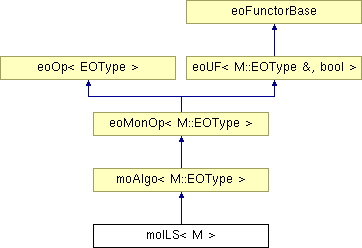
\includegraphics[height=5cm]{classmo_i_l_s}
\end{center}
\end{figure}
\subsection*{Public Member Functions}
\begin{CompactItemize}
\item 
{\bf mo\-ILS} ({\bf mo\-Algo}$<$ {\bf EOT} $>$ \&\_\-algorithm, {\bf mo\-Sol\-Continue}$<$ {\bf EOT} $>$ \&\_\-continue, {\bf mo\-Comparator}$<$ {\bf EOT} $>$ \&\_\-acceptance\_\-criterion, {\bf eo\-Mon\-Op}$<$ {\bf EOT} $>$ \&\_\-perturbation, {\bf eo\-Eval\-Func}$<$ {\bf EOT} $>$ \&\_\-full\_\-evaluation)
\begin{CompactList}\small\item\em Generic constructor. \item\end{CompactList}\item 
{\bf mo\-ILS} ({\bf mo\-Move\-Init}$<$ M $>$ \&\_\-move\_\-initializer, {\bf mo\-Next\-Move}$<$ M $>$ \&\_\-next\_\-move\_\-generator, {\bf mo\-Move\-Incr\-Eval}$<$ M $>$ \&\_\-incremental\_\-evaluation, {\bf mo\-Move\-Select}$<$ M $>$ \&\_\-move\_\-selection, {\bf mo\-Sol\-Continue}$<$ {\bf EOT} $>$ \&\_\-continue, {\bf mo\-Comparator}$<$ {\bf EOT} $>$ \&\_\-acceptance\_\-criterion, {\bf eo\-Mon\-Op}$<$ {\bf EOT} $>$ \&\_\-perturbation, {\bf eo\-Eval\-Func}$<$ {\bf EOT} $>$ \&\_\-full\_\-evaluation)
\begin{CompactList}\small\item\em Constructor for using a {\bf mo\-HC}{\rm (p.\,\pageref{classmo_h_c})} for the {\bf mo\-Algo}{\rm (p.\,\pageref{classmo_algo})}. \item\end{CompactList}\item 
{\bf mo\-ILS} ({\bf mo\-Move\-Init}$<$ M $>$ \&\_\-move\_\-initializer, {\bf mo\-Next\-Move}$<$ M $>$ \&\_\-next\_\-move\_\-generator, {\bf mo\-Move\-Incr\-Eval}$<$ M $>$ \&\_\-incremental\_\-evaluation, {\bf mo\-Tabu\-List}$<$ M $>$ \&\_\-tabu\_\-list, {\bf mo\-Aspir\-Crit}$<$ M $>$ \&\_\-aspiration\_\-criterion, {\bf mo\-Sol\-Continue}$<$ {\bf EOT} $>$ \&\_\-mo\-TS\_\-continue, {\bf mo\-Sol\-Continue}$<$ {\bf EOT} $>$ \&\_\-continue, {\bf mo\-Comparator}$<$ {\bf EOT} $>$ \&\_\-acceptance\_\-criterion, {\bf eo\-Mon\-Op}$<$ {\bf EOT} $>$ \&\_\-perturbation, {\bf eo\-Eval\-Func}$<$ {\bf EOT} $>$ \&\_\-full\_\-evaluation)
\begin{CompactList}\small\item\em Constructor for using a {\bf mo\-TS}{\rm (p.\,\pageref{classmo_t_s})} for the {\bf mo\-Algo}{\rm (p.\,\pageref{classmo_algo})}. \item\end{CompactList}\item 
{\bf mo\-ILS} ({\bf mo\-Rand\-Move}$<$ M $>$ \&\_\-random\_\-move\_\-generator, {\bf mo\-Move\-Incr\-Eval}$<$ M $>$ \&\_\-incremental\_\-evaluation, {\bf mo\-Sol\-Continue}$<$ {\bf EOT} $>$ \&\_\-mo\-SA\_\-continue, double \_\-initial\_\-temperature, {\bf mo\-Cooling\-Schedule} \&\_\-cooling\_\-schedule, {\bf mo\-Sol\-Continue}$<$ {\bf EOT} $>$ \&\_\-continue, {\bf mo\-Comparator}$<$ {\bf EOT} $>$ \&\_\-acceptance\_\-criterion, {\bf eo\-Mon\-Op}$<$ {\bf EOT} $>$ \&\_\-perturbation, {\bf eo\-Eval\-Func}$<$ {\bf EOT} $>$ \&\_\-full\_\-evaluation)
\begin{CompactList}\small\item\em Constructor for using a {\bf mo\-SA}{\rm (p.\,\pageref{classmo_s_a})} for the {\bf mo\-Algo}{\rm (p.\,\pageref{classmo_algo})}. \item\end{CompactList}\item 
bool {\bf operator()} ({\bf EOT} \&\_\-solution)
\begin{CompactList}\small\item\em Function which launches the ILS. \item\end{CompactList}\end{CompactItemize}
\subsection*{Private Types}
\begin{CompactItemize}
\item 
typedef M::EOType {\bf EOT}\label{classmo_i_l_s_y0}

\begin{CompactList}\small\item\em Alias for the type. \item\end{CompactList}\item 
typedef EOT::Fitness {\bf Fitness}\label{classmo_i_l_s_y1}

\begin{CompactList}\small\item\em Alias for the fitness. \item\end{CompactList}\end{CompactItemize}
\subsection*{Private Attributes}
\begin{CompactItemize}
\item 
{\bf mo\-Algo}$<$ {\bf EOT} $>$ \& {\bf algorithm}\label{classmo_i_l_s_r0}

\begin{CompactList}\small\item\em The solution based heuristic. \item\end{CompactList}\item 
{\bf mo\-Sol\-Continue}$<$ {\bf EOT} $>$ \& {\bf continu}\label{classmo_i_l_s_r1}

\begin{CompactList}\small\item\em The stopping criterion. \item\end{CompactList}\item 
{\bf mo\-Comparator}$<$ {\bf EOT} $>$ \& {\bf acceptance\_\-criterion}\label{classmo_i_l_s_r2}

\begin{CompactList}\small\item\em The acceptance criterion. \item\end{CompactList}\item 
{\bf eo\-Mon\-Op}$<$ {\bf EOT} $>$ \& {\bf perturbation}\label{classmo_i_l_s_r3}

\begin{CompactList}\small\item\em The perturbation generator. \item\end{CompactList}\item 
{\bf eo\-Eval\-Func}$<$ {\bf EOT} $>$ \& {\bf full\_\-evaluation}\label{classmo_i_l_s_r4}

\begin{CompactList}\small\item\em The full evaluation function. \item\end{CompactList}\end{CompactItemize}


\subsection{Detailed Description}
\subsubsection*{template$<$class M$>$ class mo\-ILS$<$ M $>$}

Iterated Local Search (ILS). 

Class which describes the algorithm for a iterated local search. 



Definition at line 50 of file mo\-ILS.h.

\subsection{Constructor \& Destructor Documentation}
\index{moILS@{mo\-ILS}!moILS@{moILS}}
\index{moILS@{moILS}!moILS@{mo\-ILS}}
\subsubsection{\setlength{\rightskip}{0pt plus 5cm}template$<$class M$>$ {\bf mo\-ILS}$<$ M $>$::{\bf mo\-ILS} ({\bf mo\-Algo}$<$ {\bf EOT} $>$ \& {\em \_\-algorithm}, {\bf mo\-Sol\-Continue}$<$ {\bf EOT} $>$ \& {\em \_\-continue}, {\bf mo\-Comparator}$<$ {\bf EOT} $>$ \& {\em \_\-acceptance\_\-criterion}, {\bf eo\-Mon\-Op}$<$ {\bf EOT} $>$ \& {\em \_\-perturbation}, {\bf eo\-Eval\-Func}$<$ {\bf EOT} $>$ \& {\em \_\-full\_\-evaluation})\hspace{0.3cm}{\tt  [inline]}}\label{classmo_i_l_s_a0}


Generic constructor. 

Generic constructor using a {\bf mo\-Algo}{\rm (p.\,\pageref{classmo_algo})}

\begin{Desc}
\item[Parameters:]
\begin{description}
\item[{\em \_\-algorithm}]The solution based heuristic to use. \item[{\em \_\-continue}]The stopping criterion. \item[{\em \_\-acceptance\_\-criterion}]The acceptance criterion. \item[{\em \_\-perturbation}]The pertubation generator. \item[{\em \_\-full\_\-evaluation}]The evaluation function. \end{description}
\end{Desc}


Definition at line 70 of file mo\-ILS.h.

References mo\-ILS$<$ M $>$::acceptance\_\-criterion, mo\-ILS$<$ M $>$::algorithm, mo\-ILS$<$ M $>$::continu, mo\-ILS$<$ M $>$::full\_\-evaluation, and mo\-ILS$<$ M $>$::perturbation.\index{moILS@{mo\-ILS}!moILS@{moILS}}
\index{moILS@{moILS}!moILS@{mo\-ILS}}
\subsubsection{\setlength{\rightskip}{0pt plus 5cm}template$<$class M$>$ {\bf mo\-ILS}$<$ M $>$::{\bf mo\-ILS} ({\bf mo\-Move\-Init}$<$ M $>$ \& {\em \_\-move\_\-initializer}, {\bf mo\-Next\-Move}$<$ M $>$ \& {\em \_\-next\_\-move\_\-generator}, {\bf mo\-Move\-Incr\-Eval}$<$ M $>$ \& {\em \_\-incremental\_\-evaluation}, {\bf mo\-Move\-Select}$<$ M $>$ \& {\em \_\-move\_\-selection}, {\bf mo\-Sol\-Continue}$<$ {\bf EOT} $>$ \& {\em \_\-continue}, {\bf mo\-Comparator}$<$ {\bf EOT} $>$ \& {\em \_\-acceptance\_\-criterion}, {\bf eo\-Mon\-Op}$<$ {\bf EOT} $>$ \& {\em \_\-perturbation}, {\bf eo\-Eval\-Func}$<$ {\bf EOT} $>$ \& {\em \_\-full\_\-evaluation})\hspace{0.3cm}{\tt  [inline]}}\label{classmo_i_l_s_a1}


Constructor for using a {\bf mo\-HC}{\rm (p.\,\pageref{classmo_h_c})} for the {\bf mo\-Algo}{\rm (p.\,\pageref{classmo_algo})}. 

\begin{Desc}
\item[Parameters:]
\begin{description}
\item[{\em \_\-move\_\-initializer}]The move initialisation (for the {\bf mo\-HC}{\rm (p.\,\pageref{classmo_h_c})}). \item[{\em \_\-next\_\-move\_\-generator}]The move generator (for the {\bf mo\-HC}{\rm (p.\,\pageref{classmo_h_c})}). \item[{\em \_\-incremental\_\-evaluation}]The partial evaluation function (for the {\bf mo\-HC}{\rm (p.\,\pageref{classmo_h_c})}). \item[{\em \_\-move\_\-selection}]The move selection strategy (for the {\bf mo\-HC}{\rm (p.\,\pageref{classmo_h_c})}). \item[{\em \_\-continue}]The stopping criterion. \item[{\em \_\-acceptance\_\-criterion}]The acceptance criterion. \item[{\em \_\-perturbation}]The pertubation generator. \item[{\em \_\-full\_\-evaluation}]The evaluation function. \end{description}
\end{Desc}


Definition at line 87 of file mo\-ILS.h.

References mo\-ILS$<$ M $>$::acceptance\_\-criterion, mo\-ILS$<$ M $>$::algorithm, mo\-ILS$<$ M $>$::continu, mo\-ILS$<$ M $>$::full\_\-evaluation, and mo\-ILS$<$ M $>$::perturbation.\index{moILS@{mo\-ILS}!moILS@{moILS}}
\index{moILS@{moILS}!moILS@{mo\-ILS}}
\subsubsection{\setlength{\rightskip}{0pt plus 5cm}template$<$class M$>$ {\bf mo\-ILS}$<$ M $>$::{\bf mo\-ILS} ({\bf mo\-Move\-Init}$<$ M $>$ \& {\em \_\-move\_\-initializer}, {\bf mo\-Next\-Move}$<$ M $>$ \& {\em \_\-next\_\-move\_\-generator}, {\bf mo\-Move\-Incr\-Eval}$<$ M $>$ \& {\em \_\-incremental\_\-evaluation}, {\bf mo\-Tabu\-List}$<$ M $>$ \& {\em \_\-tabu\_\-list}, {\bf mo\-Aspir\-Crit}$<$ M $>$ \& {\em \_\-aspiration\_\-criterion}, {\bf mo\-Sol\-Continue}$<$ {\bf EOT} $>$ \& {\em \_\-mo\-TS\_\-continue}, {\bf mo\-Sol\-Continue}$<$ {\bf EOT} $>$ \& {\em \_\-continue}, {\bf mo\-Comparator}$<$ {\bf EOT} $>$ \& {\em \_\-acceptance\_\-criterion}, {\bf eo\-Mon\-Op}$<$ {\bf EOT} $>$ \& {\em \_\-perturbation}, {\bf eo\-Eval\-Func}$<$ {\bf EOT} $>$ \& {\em \_\-full\_\-evaluation})\hspace{0.3cm}{\tt  [inline]}}\label{classmo_i_l_s_a2}


Constructor for using a {\bf mo\-TS}{\rm (p.\,\pageref{classmo_t_s})} for the {\bf mo\-Algo}{\rm (p.\,\pageref{classmo_algo})}. 

\begin{Desc}
\item[Parameters:]
\begin{description}
\item[{\em \_\-move\_\-initializer}]The move initialisation (for the {\bf mo\-TS}{\rm (p.\,\pageref{classmo_t_s})}). \item[{\em \_\-next\_\-move\_\-generator}]The move generator (for the {\bf mo\-TS}{\rm (p.\,\pageref{classmo_t_s})}). \item[{\em \_\-incremental\_\-evaluation}]The partial evaluation function (for the {\bf mo\-TS}{\rm (p.\,\pageref{classmo_t_s})}). \item[{\em \_\-tabu\_\-list}]The tabu list (for the {\bf mo\-TS}{\rm (p.\,\pageref{classmo_t_s})} !!!!). \item[{\em \_\-aspiration\_\-criterion}]The aspiration criterion (for the {\bf mo\-TS}{\rm (p.\,\pageref{classmo_t_s})}). \item[{\em \_\-mo\-TS\_\-continue}]The stopping criterion (for the {\bf mo\-TS}{\rm (p.\,\pageref{classmo_t_s})}). \item[{\em \_\-continue}]The stopping criterion. \item[{\em \_\-acceptance\_\-criterion}]The acceptance criterion. \item[{\em \_\-perturbation}]The pertubation generator. \item[{\em \_\-full\_\-evaluation}]The evaluation function. \end{description}
\end{Desc}


Definition at line 108 of file mo\-ILS.h.

References mo\-ILS$<$ M $>$::acceptance\_\-criterion, mo\-ILS$<$ M $>$::algorithm, mo\-ILS$<$ M $>$::continu, mo\-ILS$<$ M $>$::full\_\-evaluation, and mo\-ILS$<$ M $>$::perturbation.\index{moILS@{mo\-ILS}!moILS@{moILS}}
\index{moILS@{moILS}!moILS@{mo\-ILS}}
\subsubsection{\setlength{\rightskip}{0pt plus 5cm}template$<$class M$>$ {\bf mo\-ILS}$<$ M $>$::{\bf mo\-ILS} ({\bf mo\-Rand\-Move}$<$ M $>$ \& {\em \_\-random\_\-move\_\-generator}, {\bf mo\-Move\-Incr\-Eval}$<$ M $>$ \& {\em \_\-incremental\_\-evaluation}, {\bf mo\-Sol\-Continue}$<$ {\bf EOT} $>$ \& {\em \_\-mo\-SA\_\-continue}, double {\em \_\-initial\_\-temperature}, {\bf mo\-Cooling\-Schedule} \& {\em \_\-cooling\_\-schedule}, {\bf mo\-Sol\-Continue}$<$ {\bf EOT} $>$ \& {\em \_\-continue}, {\bf mo\-Comparator}$<$ {\bf EOT} $>$ \& {\em \_\-acceptance\_\-criterion}, {\bf eo\-Mon\-Op}$<$ {\bf EOT} $>$ \& {\em \_\-perturbation}, {\bf eo\-Eval\-Func}$<$ {\bf EOT} $>$ \& {\em \_\-full\_\-evaluation})\hspace{0.3cm}{\tt  [inline]}}\label{classmo_i_l_s_a3}


Constructor for using a {\bf mo\-SA}{\rm (p.\,\pageref{classmo_s_a})} for the {\bf mo\-Algo}{\rm (p.\,\pageref{classmo_algo})}. 

\begin{Desc}
\item[Parameters:]
\begin{description}
\item[{\em \_\-random\_\-move\_\-generator}]The random move generator (for the {\bf mo\-SA}{\rm (p.\,\pageref{classmo_s_a})}). \item[{\em \_\-incremental\_\-evaluation}]The partial evaluation function (for the {\bf mo\-SA}{\rm (p.\,\pageref{classmo_s_a})}). \item[{\em \_\-mo\-SA\_\-continue}]The stopping criterion (for the {\bf mo\-SA}{\rm (p.\,\pageref{classmo_s_a})}). \item[{\em \_\-initial\_\-temperature}]The initial temperature (for the {\bf mo\-SA}{\rm (p.\,\pageref{classmo_s_a})}). \item[{\em \_\-cooling\_\-schedule}]The cooling schedule (for the {\bf mo\-SA}{\rm (p.\,\pageref{classmo_s_a})}). \item[{\em \_\-continue}]The stopping criterion. \item[{\em \_\-acceptance\_\-criterion}]The acceptance criterion. \item[{\em \_\-perturbation}]The pertubation generator. \item[{\em \_\-full\_\-evaluation}]The evaluation function. \end{description}
\end{Desc}


Definition at line 130 of file mo\-ILS.h.

References mo\-ILS$<$ M $>$::acceptance\_\-criterion, mo\-ILS$<$ M $>$::algorithm, mo\-ILS$<$ M $>$::continu, mo\-ILS$<$ M $>$::full\_\-evaluation, and mo\-ILS$<$ M $>$::perturbation.

\subsection{Member Function Documentation}
\index{moILS@{mo\-ILS}!operator()@{operator()}}
\index{operator()@{operator()}!moILS@{mo\-ILS}}
\subsubsection{\setlength{\rightskip}{0pt plus 5cm}template$<$class M$>$ bool {\bf mo\-ILS}$<$ M $>$::operator() ({\bf EOT} \& {\em \_\-solution})\hspace{0.3cm}{\tt  [inline]}}\label{classmo_i_l_s_a4}


Function which launches the ILS. 

The ILS has to improve a current solution. As the {\bf mo\-SA}{\rm (p.\,\pageref{classmo_s_a})}, the {\bf mo\-TS}{\rm (p.\,\pageref{classmo_t_s})} and the {\bf mo\-HC}{\rm (p.\,\pageref{classmo_h_c})}, it can be used for HYBRIDATION in an evolutionnary algorithm.

\begin{Desc}
\item[Parameters:]
\begin{description}
\item[{\em \_\-solution}]a current solution to improve. \end{description}
\end{Desc}
\begin{Desc}
\item[Returns:]true. \end{Desc}


Definition at line 146 of file mo\-ILS.h.

References mo\-ILS$<$ M $>$::acceptance\_\-criterion, mo\-ILS$<$ M $>$::algorithm, mo\-ILS$<$ M $>$::continu, mo\-ILS$<$ M $>$::EOT, mo\-ILS$<$ M $>$::full\_\-evaluation, and mo\-ILS$<$ M $>$::perturbation.

The documentation for this class was generated from the following file:\begin{CompactItemize}
\item 
mo\-ILS.h\end{CompactItemize}
